
\documentclass[11pt]{article}
\usepackage[margin=1in]{geometry}
\usepackage{amsmath,amssymb}
\usepackage{graphicx}
\usepackage{booktabs}
\usepackage{xcolor}
\usepackage[authoryear,round]{natbib}
\usepackage[colorlinks=true,linkcolor=blue,citecolor=blue,urlcolor=blue]{hyperref}

% ADS journal macros used by refs.bib (a journal class defines them; \providecommand leaves those)
\providecommand{\mnras}{MNRAS}\providecommand{\apj}{ApJ}\providecommand{\apjs}{ApJS}\providecommand{\aj}{AJ}
\providecommand{\apjl}{ApJL}\providecommand{\aap}{A\&A}\providecommand{\jcap}{JCAP}
\providecommand{\pasp}{PASP}\providecommand{\araa}{ARA\&A}\providecommand{\prd}{Phys.~Rev.~D}
\providecommand{\nat}{Nature}\providecommand{\physrep}{Phys.~Rep.}\providecommand{\na}{New Astron.}
\newcommand{\todo}[1]{\textcolor{red}{[TODO: #1]}}
\newcommand{\draft}[1]{\textcolor{orange}{[draft: #1]}}
\newcommand{\chat}{\hat{c}}
\newcommand{\hmpc}{\,h\,\mathrm{Mpc}^{-1}}
\newcommand{\mpch}{\,\mathrm{Mpc}/h}
\newcommand{\xv}{x_{\rm V}}
\newcommand{\Ndir}{N_{\rm OT}}
\newcommand{\T}{^{\mathsf T}}
\newcommand{\placeholder}[1]{\fbox{\parbox[c][5cm][c]{0.9\linewidth}{\centering\textcolor{red}{To make:} #1}}}

\title{Moment closures against ray tracing for modeling reionization}
\author{\todo{authors}}
\date{Outline, 2026-11-06}

\begin{document}
\maketitle

\begin{abstract}
We compare reionizations simulations run different moment closures, such as M1 and OTVET, with full radiative transfer all implemented ontop of the same hydro-dark matter code.  For the structure of reionization, all represent the structure well enough for radiative transfer to not be a major modeling uncertainty (and significantly better than 21cmFast).  OTVET and espeically M1 do not capture well the photoionization fluctuations after reionization. We propose a few \todo{two?} simple closure schemes that perform significantly better.  However, we show that even M1 likely captures $\tau_{\rm eff}$ fluctuations in the Ly$\alpha$ with sufficient accuracy.
\end{abstract}

%======================================================================
\section{Introduction}
Moment methods are the workhorse of radiative transfer in large reionization
simulations. M1 underlies RAMSES-RT \citep{rosdahl13}, ATON
\citep{aubert08} and AREPO-RT \citep{kannan19}, and through AREPO-RT the
Thesan simulations \citep{kannan22}; the optically thin variable Eddington
tensor (OTVET; \citealt{gnedin01}) underlies the CROC simulations
\citep{gnedin14}. Before overlap, the transfer sets the morphology of reionization that
21\,cm experiments will map \citep{Furlanetto2006}; after it, the $\Gamma_{\rm HI}$
these methods return sets the Ly$\alpha$ forest, the mean free path, the
scatter in $\tau_{\rm eff}$ \citep{davies16,davies17}; so closure errors become
errors in the observables.

The closures have known problems. M1 carries one flux direction per cell,
so crossing beams merge and the proximity zones of individual sources are
lost. The optically thin tensor ignores intervening absorbers, so it casts
no shadows \citep{gnedin01,petkova09}, and its normalisation depends on box
size \citep{wu21}. \citet{gnedin25} showed that CROC and Thesan disagree on the transfer function between
$\Gamma_{\rm HI}$ and the sources, and he noted that no ray-tracing
calculation exists to decide between them.

The natural improvement is to attenuate the tensor by the intervening
absorbers, as has been done with long characteristics \citep{finlator09},
short characteristics \citep{davis12} and tree-based column densities
\citep{pawlik08,clark12,hopkins20,wunsch21}, or two go to second-order.  However, second-order closures are
unstable \citep{gnedinkatz26}.

Here we test first order closure ideas against the exact answer. (1) One code holds every
closure and adaptive ray tracing \citep{trac07}, with all other physics
shared, so differences between runs come from the transfer alone. (2) We
measure the true Eddington tensor from the rays and compare each closure
with it. (3) We study three closures, one a new HI-attenuated tensor built
by cone tracing.

%======================================================================
\section{Simulations and radiative transfer}


All runs use a C++ port of the cosmological radiation-hydrodynamics code
of \citet{trac07}, which couples a
particle-mesh (PM) $N$-body solver for the dark matter, an Eulerian solver
for the gas, and the transfer of ionizing radiation in five frequency
groups with non-equilibrium hydrogen and helium chemistry and
photoheating. With its original settings the port reproduces the Fortran
code bit for bit on a set of validation problems. %The runs here enable a set of bookkeeping and physics corrections to the original (among them photon-conserving ray deposition). They also replace its moving-frame hydrodynamics scheme with an unsplit MUSCL--Hancock scheme with HLLC fluxes and a dual-energy formulation \citep{toro09}, which removes the spurious heating of cold, supersonically moving gas.

The comparison uses one uniform suite of seven runs that differ only in
the radiative transfer (Table~\ref{tab:runs}). The box is $40\mpch$ on a
side, with $512^3$ gas and RT cells ($78\,h^{-1}$\,kpc) and $1024^3$ dark
matter particles of $6.4\times10^6\,M_\odot$, whose forces are computed on
a $2048^3$ PM mesh. The cosmology is $\Omega_m=0.27$,
$\Omega_\Lambda=0.73$, $\Omega_b=0.045$, $h=0.70$, $\sigma_8=0.80$ and
$n_s=0.96$. The initial conditions are a Zel'dovich realization at $z=100$
of the no-wiggle linear power spectrum of \citet{eisenstein98}..

Sources are the friends-of-friends halos (linking length 0.2) found on the
fly at every hydro step, down to 20 particles
($1.3\times10^8\,M_\odot$). Each halo's UV luminosity comes from abundance
matching observed UV luminosity functions to a Sheth--Tormen mass function
refit to the friends-of-friends halos of this box
\citep{sheth99,bouwens21,bouwens22,donnan24,atek26}. Below the turnover,
this gives $L_{\rm UV}\propto M^{1.43\textrm{--}1.46}$ at $z=7$--5.7. The
ionizing photon production efficiency is
$\log\xi_{\rm ion}=25.38$ \citep{pahl25}, and the escape fraction is
$f_{\rm esc}(z)=f_6\,[(1+z)/7]^{2.5}$ with $f_6=0.11$, chosen so that
reionization ends with ionized fraction $\xv=0.99$ at $z\approx5.6$, a redshift scaling motivated by \todo{cite D'Aloisio in prep}. 
% f6 = 0.11 and the continuous c-hat schedule: the suite's launch record
% (NewRadHydroCode docs/STATUS.md); the table in rt_suite_512.md S1 is stale.

All runs use case-B recombination with on-the-spot absorption of the
recombination photons, except one ray run with case-A recombination and
the recombination radiation transported (``rays, case A + RR''). %As in the original code, cooling is suppressed above 200 times the mean density, and a cell denser than 50 times the mean (overdensity $\delta>50$) removes only a fraction $e^{-(\delta-50)/50}$ of the photons its photoionizations use, so the densest gas neither consumes nor shields much radiation.
The reduced speed of light follows the volume-weighted ionized fraction
$x$ of the previous hydro step. It is piecewise linear through
$(x,\chat/c)=(0.125,0.1)$, $(0.375,0.2)$, $(0.625,0.3)$ and $(0.875,0.5)$,
and constant outside them, a schedule chosen to achieve a converged ionization history to better than $\Delta z<0.1$.  Every $\Gamma_{\rm HI}$ statistic uses
$\Gamma_{\rm HI}$ averaged over the RT substeps of the hydro step, which
removes most of the rays' sampling noise. Since the runs share their
initial conditions and sources, and their histories agree to within 0.1
in $z$, we compare them at fixed redshift.
%Making it continuous in $x$ avoids the jumps in $\Gamma_{\rm HI}$ that a stepped schedule causes each time it switches. Radiation is redshifted by the distance it travels rather than by elapsed time, which is appropriate for $\chat<c$. The radiative transfer starts at $z=15$ and the runs end at $z=5$.


The seven runs differ only in how the radiation is transported.

\paragraph{Rays.} The reference. Each source emits rays along HEALPix
directions \citep{gorski05}, which split as they travel so that every cell
they reach is crossed by several rays \citep{abel02,trac07}, and deposit
their photoionizations cell by cell, conserving photons. One comparison run uses
case-B recombination, the other case A with the recombination radiation
transported.

\paragraph{Moment methods.} For each frequency group, we evolve the photon
density $N$ and the flux $\chat\,\mathbf F$,
\begin{align}
\partial_t N + \chat\,\nabla\cdot\mathbf F &= S - \chat\kappa N,\\
\partial_t \mathbf F + \chat\,\nabla\cdot(\mathsf D\,N) &= -\chat\kappa \mathbf F,
\end{align}
with a first-order Godunov scheme using global Lax--Friedrichs fluxes of
wave speed $\chat$. The sources $S$, the absorption $\kappa$ and the
redshifting are those of the ray runs. The methods differ only in the
Eddington tensor $\mathsf D$ (trace 1). M1 and OTVET are the two closures
in common use in reionization simulations; we also consider three new
ones, described in \S\ref{sec:closures}:
\begin{itemize}
\item \textbf{M1} \citep{levermore84} takes $\mathsf D$ from the local
  reduced flux $f=|\mathbf F|/N$:
  $\mathsf D=\frac{1-\chi}{2}\mathsf I+\frac{3\chi-1}{2}\hat{\mathbf u}\hat{\mathbf u}\T$,
  with $\chi=(3+4f^2)/(5+2\sqrt{4-3f^2})$ and $\hat{\mathbf u}=\mathbf F/|\mathbf F|$.
The advantage of M1 is that it needs only each cell's own moments and is exact for a single beam,
  which makes it cheap and local. With one flux direction
  per cell, however, it cannot represent light arriving from several
  directions, which it merges and diffuses.
\item \textbf{OTVET} takes $\mathsf D=\mathsf h=\mathsf S/{\rm tr}\,\mathsf S$,
  the optically thin Eddington tensor of the current sources
  \citep{gnedin01}, applied here to the whole radiation field,
  \begin{equation}
  \mathsf S(\mathbf x)=\sum_s L_s\,\frac{\mathbf d_s\mathbf d_s\T}{|\mathbf d_s|^4},
  \qquad \mathbf d_s=\mathbf x-\mathbf x_s,
  \label{eqn:otvet}
  \end{equation}
  with each source $s$ of luminosity $L_s$ at its nearest periodic image,
  computed by FFT once per hydro step. The tensor is non-local and exact
  around an isolated source, so it keeps the radial geometry of the
  light. It ignores absorption, though, and counts sources only out to
  half a box, so applied to the whole field it becomes too anisotropic
  once the mean free path exceeds the box \citep{wu21}. \citet{gnedin01}
  and CROC \citep{gnedin14} apply it only to a local part of the field
  and carry the rest as an isotropic background, whose share is set by a
  global opacity; our OTVET runs, like the analysis of \citet{wu21}, have
  no background component.
\item \textbf{Split} (new): a local version of the background
  decomposition of \citet{gnedin01} and CROC \citep{gnedin14}. The OTVET
  tensor is applied only to the photons the optically thin approximation
  accounts for, $N_{\rm OT}$, and the rest of the cell's photons are
  isotropic, $\mathsf D=\mathsf I/3+\min(1,N_{\rm OT}/N)\,(\mathsf h-\mathsf I/3)$.
  Where those schemes set the isotropic share with a global opacity or an
  observed mean free path and transport it as a second field, the split
  takes it cell by cell from the solution's own photons, with no free
  parameter and at no extra cost.
\item \textbf{Screen} (new): Rather than the optically thin approximation as in equation~\ref{eqn:otvet}, $\mathsf h$ from the sources' light
  attenuated by $e^{-r/\lambda}$ and summed over all periodic images, with
  $\lambda$ the photons' mean path from the photon budget. This is the
  remedy \citet{wu21} propose: attenuating at the mean free path gives the
  right anisotropy on average, but with one $\lambda$ for every
  direction.  Here $\lambda$ is calculated from the photon budget at the start of each
hydro step, $\lambda=\sum N/(\dot N_{\rm inj}\,\Delta t_{\rm RT})$: the
photons the solution holds divided by those the sources inject per RT
substep. Since a substep is one cell of light travel, this is $\chat$
times the mean photon lifetime, so that the screened light,
$\int e^{-r/\lambda}/(4\pi r^2)\,d^3r=\lambda$ per unit emission, totals
the photons in the box.
\item \textbf{Cone} (new): our most sophisticated closure. The cone tensor therefore attenuates
  each source's light by the HI along the way. Receivers, one every 4
  cells, each cast 192 HEALPix cones (half-opening $\approx8^\circ$). Each
  cone is marched outward through coarsened copies (mip-maps) of the
  emissivity and of the HI column, sampling at each step the level whose
  cells match the cone's width, so the number of steps grows only
  logarithmically with distance and the cost does not depend on the
  number of sources. Along the way the light is attenuated by
  $T=\sum_g W_g\,e^{-\sigma_g N_{\rm HI}}$, the transmission of the
  source spectrum weighted by each group's contribution to
  $\Gamma_{\rm HI}$. The optical depth of each cell is capped at unity,
  a stand-in for the covering fraction of absorbers smaller than a cone.
  The march continues through the periodic images to 8 box lengths.
  Within $r_c=8$ cells of the receiver, where cones are narrower than a
  cell, the thin tensor (by FFT) is used instead. After overlap the
  diffuse IGM barely attenuates the cones, so their light is cut by an
  extra $e^{-s/\lambda_x}$, with $\lambda_x$ set each hydro step so that
  the light in the ionized cells equals the photons the solution holds
  there. The receivers' tensors are interpolated to every cell and blended
  with the split on scales below $\sigma=4$ cells,
  $\mathsf h=\mathsf h_{\rm split}+G_\sigma*(\mathsf h_{\rm cone}-\mathsf h_{\rm split})$,
  because the cones are too coarse to resolve structure within a few
  cells of a source. The cone tensor costs about 4 times the thin tensor
  per hydro step, and 7\% more wall time in the 512$^3$ runs.
\end{itemize}
The walltime for all the simple closures are about 10 hours (cone takes an extra $\approx 45$ minutes), and the runs with rays take about 24 hours, where all runs were run on 192 cores on the Hyak Klone machine.  The time computing the Eddington tensor time per step at 256$^3$ is 0.7\,s for OTVET, 1.2\,s for screen, and 3.2\,s for the cone.

We also will compare the radiative transfer models agains 21cmFAST. \todo{describe}


%======================================================================
\section{Results}
\subsection{Morphology of reionization}


\begin{figure}[h]
\centering
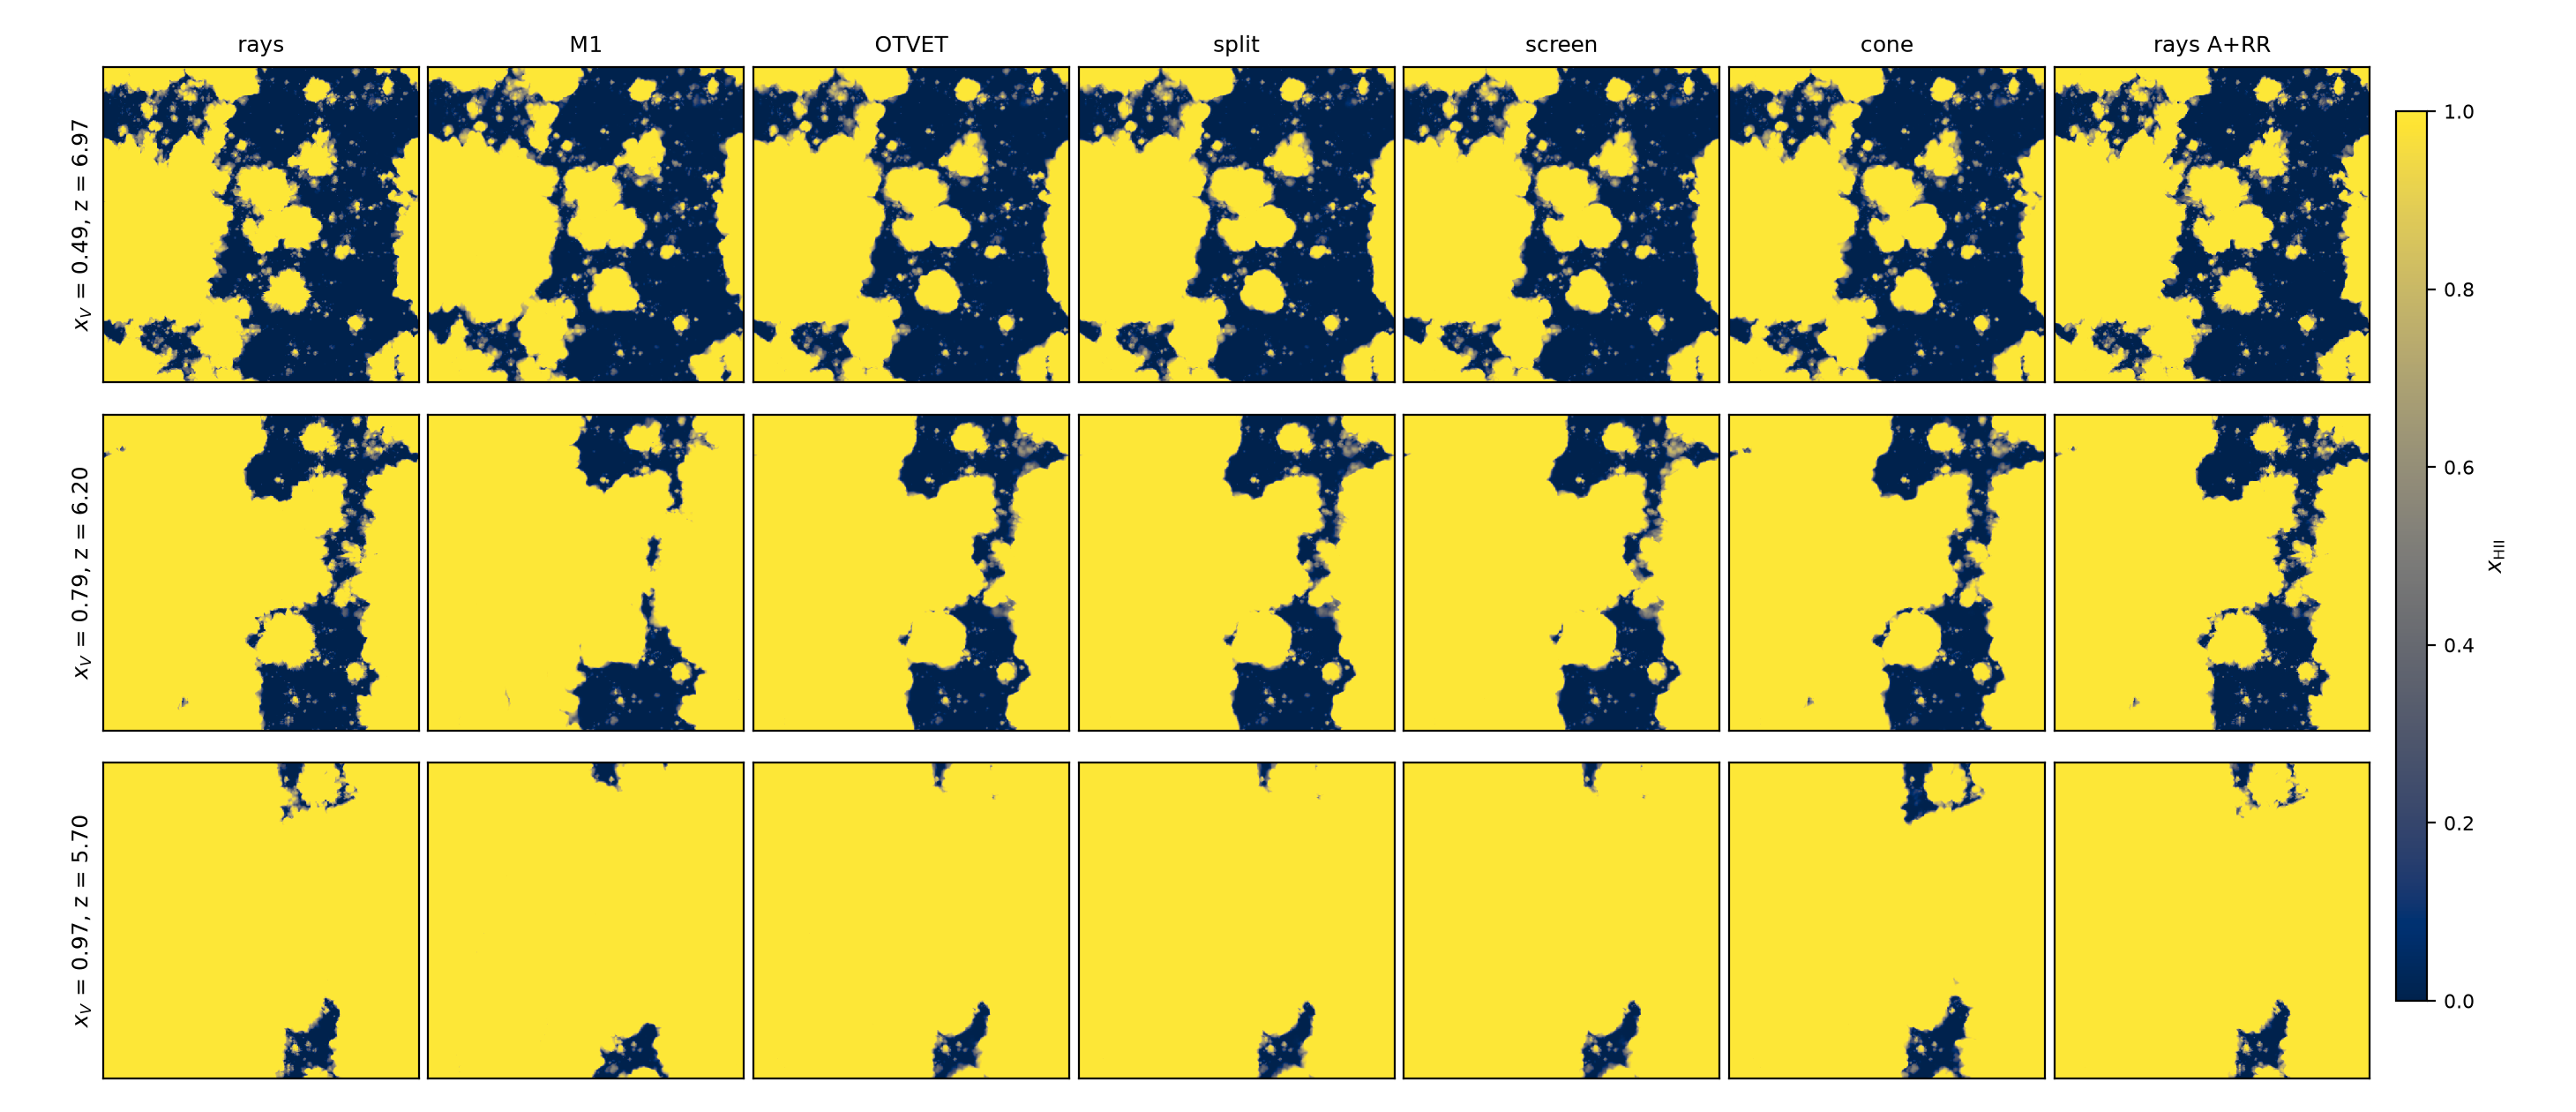
\includegraphics[width=\linewidth]{figures/fig1_maps_xHII_draft.png}
\caption{$x_{\rm HII}$ in 8-cell ($0.625\mpch$) slabs through the box
middle at $z=6.97$, 6.20 and 5.70 ($\xv=0.49$, 0.79, 0.97 in the rays):
the rays, M1, OTVET, the cone, and 21cmFAST's excursion-set
criterion on the suite's own gas density ($R_{\rm max}=15$\,Mpc), with
mass-dependent sources matched to the suite's (\texttt{E-INTEGRAL},
$\alpha_\star=a(z)-1=0.43$--0.46 from the abundance matching,
$\alpha_{\rm esc}=0$, the normalisation chosen at each $z$ to give the
rays' $\xv$). \draft{cut by \texttt{scripts/fig1\_compose\_draft.py} from
NewRadHydroCode \texttt{taueff\_21cmfast\_fig8\_maps.png} (branch
\texttt{21cmfast-mass-sources}, 61b8312). Final from the cubes:
\texttt{rt\_suite\_figures.py} with the \texttt{excursion\_set.py} output
as one more run (it needs an option for runs without $\Gamma$).}}
\label{fig:maps}
\end{figure}


\begin{figure}[h]
\centering
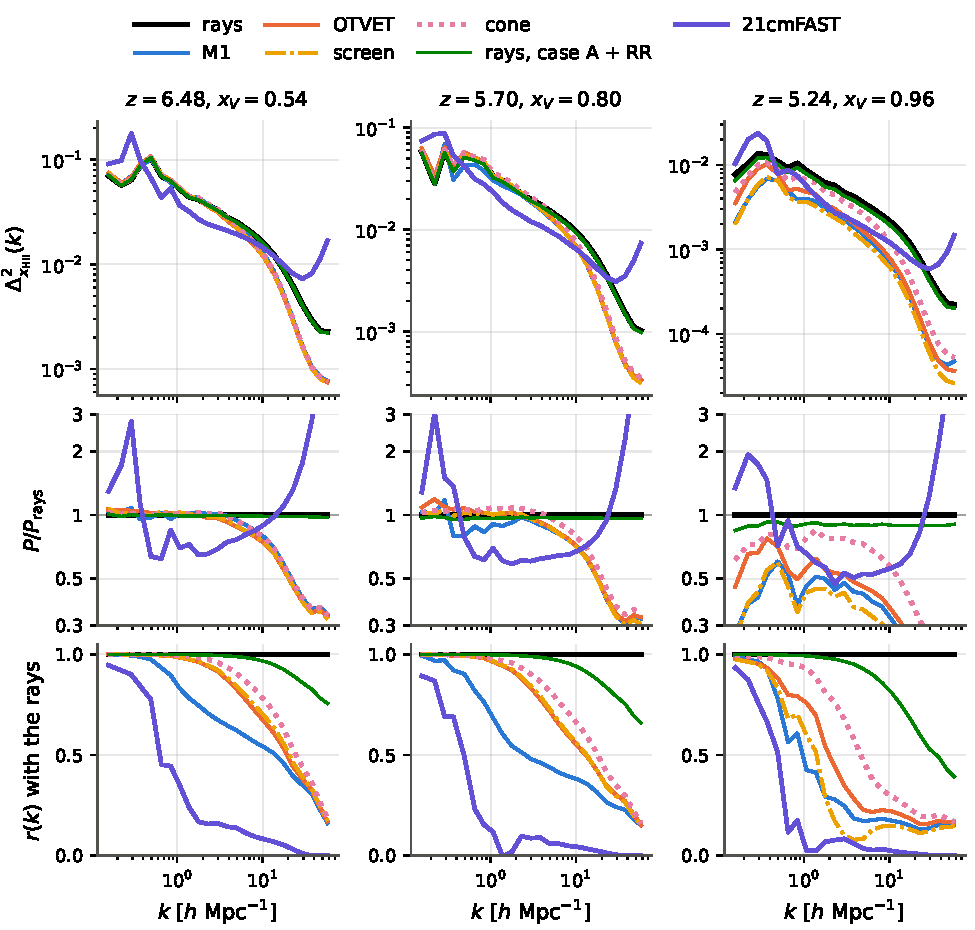
\includegraphics[width=\linewidth]{figures/fig2_pk_xHII.pdf}
\caption{$\Delta^2$ of $x_{\rm HII}$ (top), the ratio to the rays (middle)
and the cross-correlation coefficient with the rays (bottom) at $z=6.97$,
6.20 and 5.70: every run and 21cmFAST (\texttt{scripts/fig\_pk.py}).}
\label{fig:pkx}
\end{figure}






Figure~\ref{fig:maps} shows the ionized fraction in a $0.625\mpch$ deep slab through the
box at three stages of reionization. All the RT methods agree on where
the ionized regions are: the bubbles grow around the same source
clusters, and on scales above a few Mpc the $x_{\rm HII}$ fields are
nearly identical. The methods differ at the fronts and in the
last neutral islands. With the rays' $\xv$ at each redshift matched to
within 1\% by all the methods.  % 1.8\% of the cells differ from the rays by more than 0.5 in $x_{\rm HII}$ for the cone at $z=6.97$ and 6.20, 2.8--3.0\% for OTVET, and 6.6--7.8\% for M1.

 M1's local closure merges the
light of several sources into one flux per cell and diffuses it, so the
fronts lose the geometry leading to rounder fronts and that are most geometrically distinct from the other methods. OTVET keeps that
geometry, since its tensor points at the sources, but it illuminates
every front from all sides at the optically thin rate. Its fronts are
more diffuse than rays, and its last islands are eroded early. The cone, which attenuates the light by
the HI along each direction, produces a very similar morphology to the rays' at every stage.

21cmFAST, applied to the same density field with sources matched to the
suite's, differs far more from the rays than any RT method does.  21cmFast does essentially no radiative transfer, assigning ionization based on smoothing the distribution of emission and asking if there are enough photons on any sphere around a pixel to ionize that sphere, and marking it as ionized if the answer is `yes'. It
ionizes the largest overdense region completely and early, while many of
the isolated bubbles the rays grow around individual sources are absent.

Figure~\ref{fig:pkx} quantifies these differences with the power spectrum
of $x_{\rm HII}$, its ratio to the rays' and the cross-correlation
coefficient $r(k)$ with the rays. On large scales every RT method has the
rays' power to within 10\% until $\xv\approx0.8$. The cross-correlation
then separates the methods. M1 decorrelates first: $r=0.86$ already at
$k\approx1\hmpc$ at $\xv=0.49$, falling to 0.57 at $\xv=0.97$, the
displaced fronts of Figure~\ref{fig:maps}. On smaller scales
($k\approx5\hmpc$) the cone stays the closest, with $r=0.92$, 0.86 and
0.65 at $\xv=0.49$, 0.79 and 0.97, against 0.85, 0.69 and 0.30 for OTVET
and 0.65, 0.43 and 0.26 for M1; the split equals OTVET here, since it
only acts after overlap. At the end of reionization ($\xv=0.97$) OTVET,
whose islands erode early, has half the rays' power at $k\gtrsim1\hmpc$,
while the cone has 1.2--1.3 times the rays' at $k=1$--$5\hmpc$: its
islands are sharper. Recombination radiation (case A + RR) changes the
morphology less than any closure, with $r\ge0.99$ at $k\le2\hmpc$
throughout. 21cmFAST has 1.6--3.1 times the rays' power at
$k\approx0.2\hmpc$, its ionized regions too clustered on the largest
scales, and 0.5--0.8 times on scales of 1--$3\hmpc$, and its $r(k)$
falls below 0.5 by $k\approx0.5$--$1\hmpc$.

\subsection{Fluctuations in the photoionization rate}


\begin{figure}[h]
\centering
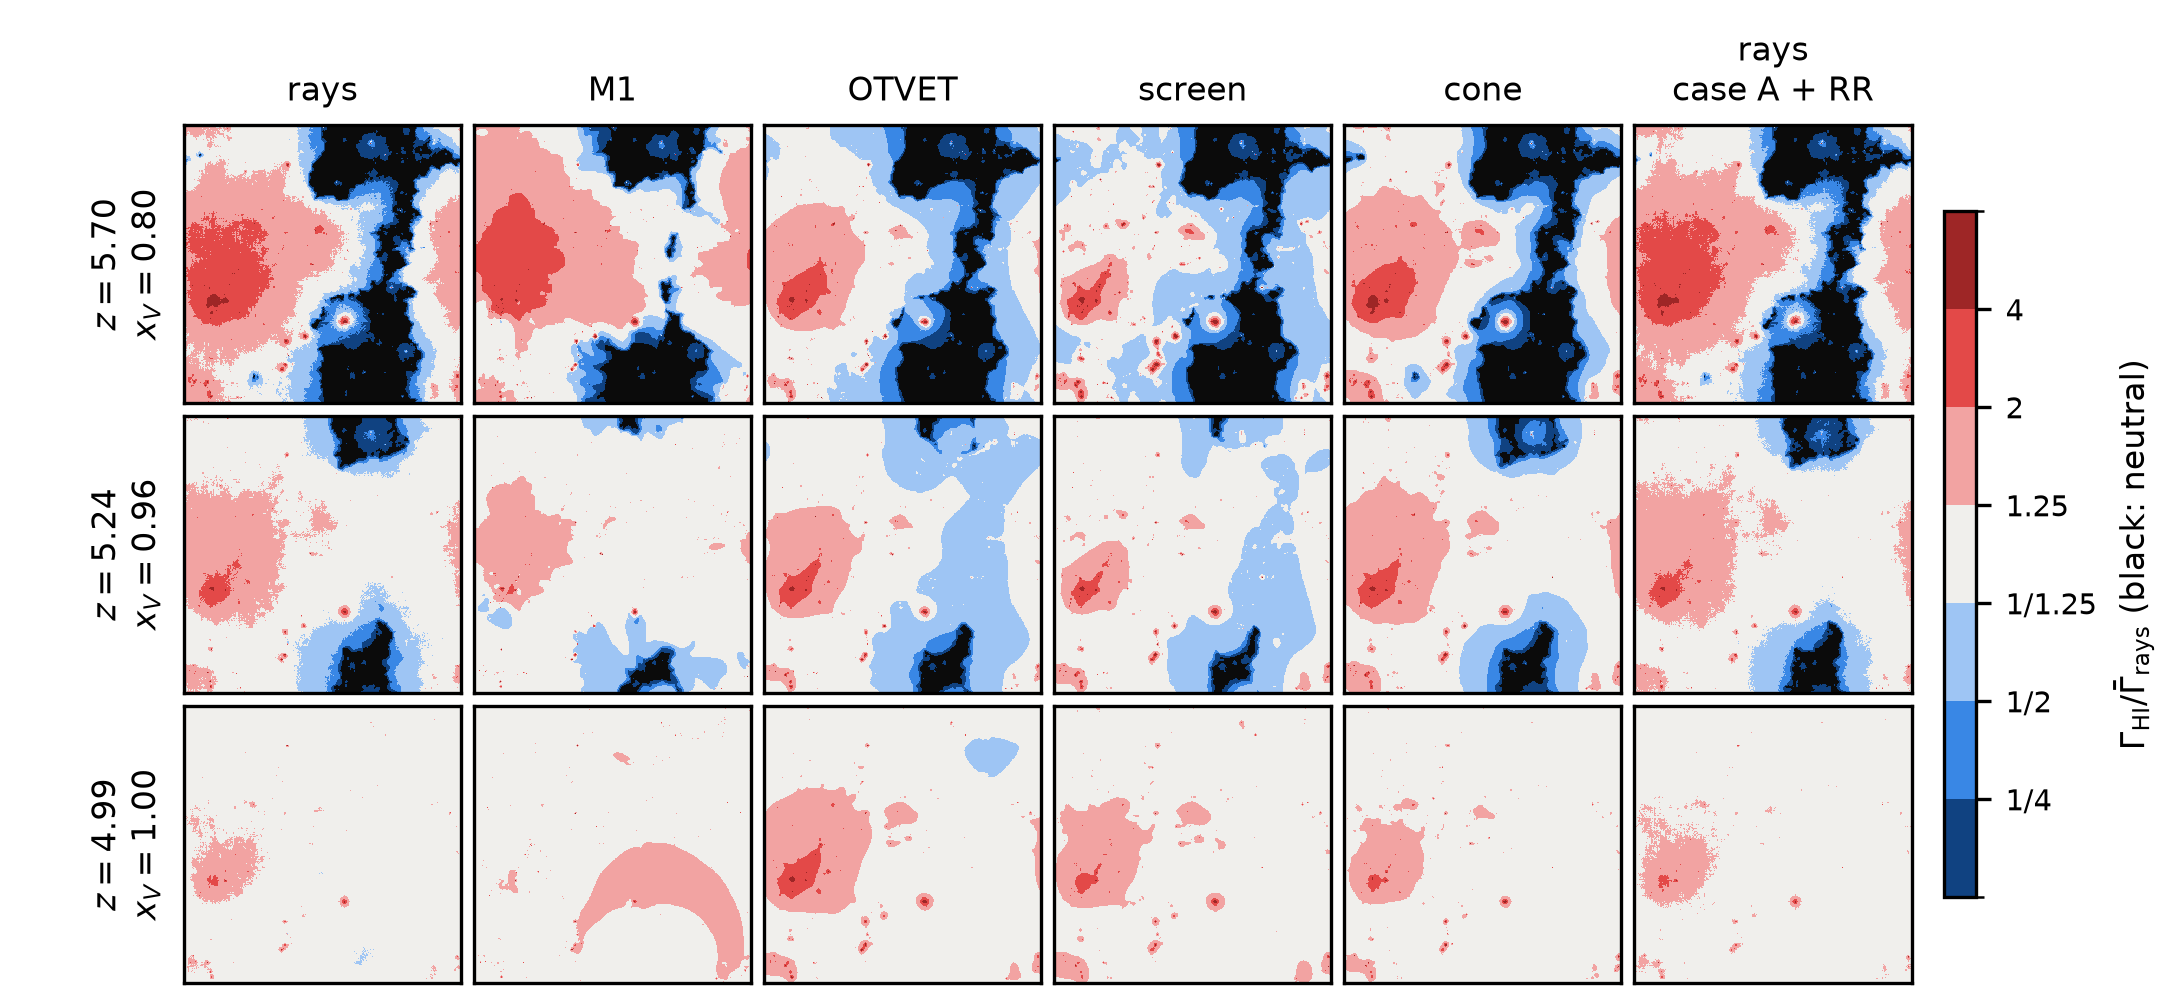
\includegraphics[width=\linewidth]{figures/fig3_gamma_maps.png}
\caption{\draft{panels cut from \texttt{rt\_suite\_512\_maps\_gamma.png},
relabelled by \texttt{scripts/fig3\_gamma\_maps.py}.}
$\Gamma_{\rm HI}$ (\texttt{gammaHI\_avg}) in 8-cell slabs through the box
middle at $z=6.20$, 5.70 and 4.99 ($\xv=0.79$, 0.97, 1.00 in the rays), all
seven runs. Final: regenerated with \texttt{rt\_suite\_figures.py
--xv-gamma 0.8,0.97,1.0}; possibly a zoom on a source cluster and
$\Gamma/\langle\Gamma\rangle$ on a narrower range to show the proximity
zones.}
\label{fig:mapsg}
\end{figure}

\begin{figure}[h]
\centering
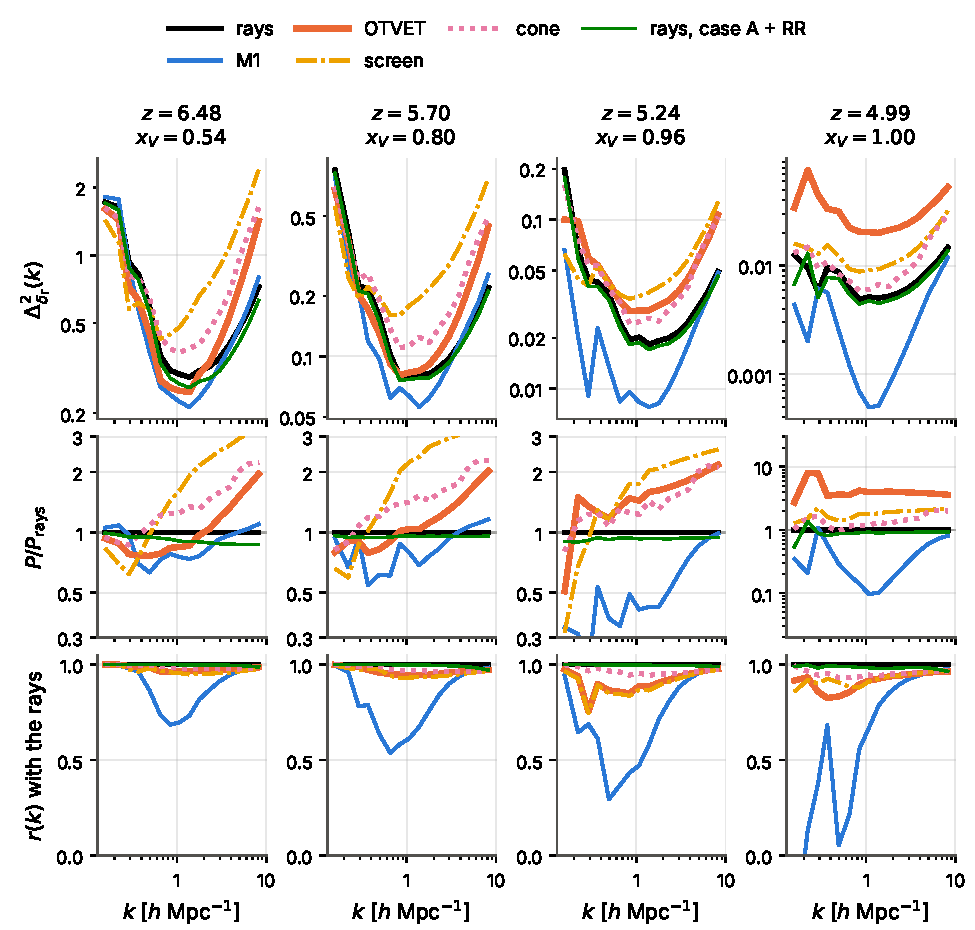
\includegraphics[width=\linewidth]{figures/fig4_pk_gamma.pdf}
\caption{As Fig.~\ref{fig:pkx}, for $\delta_\Gamma$ at $\xv=0.49$, 0.79,
0.97 and after overlap (\texttt{scripts/fig\_pk.py}). \draft{Final: $\Delta^2$ of
$\delta_\Gamma$ (\texttt{gammaHI\_avg}), the ratio to the rays and $r(k)$
at $z\approx6.0$, 5.5 and 5.0 (snapshots 5.98, 5.49, 4.99), every
method and the case A + RR rays (needs a
\texttt{--z} option in \texttt{rt\_suite\_figures.py}).}}
\label{fig:pkg}
\end{figure}


The closures differ more in the photoionization rate than in the
ionized fraction. Figure~\ref{fig:mapsg} shows $\Gamma_{\rm HI}$ in the
same slab. The mean rate is set by the photon budget and agrees between
the methods: the median $\Gamma_{\rm HI}$ of the ionized cells is within
10\% of the rays' from $z=12$ to 5. Its distribution is not. Inside the
bubbles the rays, the cone and the case A + RR rays show a rate that
falls away from each source, the proximity zones resolved. M1 fills its
bubbles with a nearly uniform rate: once a cell's photons are mostly a
nearly isotropic background, a source's flux is a small part of the
cell's, M1's closure becomes almost isotropic, and the source's light
diffuses instead of streaming. OTVET and the split have the rays'
structure inside the bubbles but at a lower level, and the screen gives
a mottled field during reionization, its single attenuation length
over-weighting the nearest sources. After overlap ($z=4.99$) all the
runs are smooth except OTVET, which keeps bright patches around the
source clusters. The one-point distribution shows the same: between its
0.1 and 99.9 percentiles, $\Gamma/\langle\Gamma\rangle$ in ionized
cells spans 0.81--1.85 for the rays, 0.92--1.93 for the cone, 0.94--1.26
for M1, which has no proximity zones, and 0.65--4.2 for OTVET.

Figure~\ref{fig:pkg} shows the power spectrum of
$\delta_\Gamma=\Gamma_{\rm HI}/\langle\Gamma_{\rm HI}\rangle-1$ and its
cross-correlation with the rays. During reionization ($\xv=0.49$ and
0.79) all the OTVET variants follow the rays closely ($r\ge0.95$ at
$k\le2\hmpc$ and the power within 30\%), except the screen, with twice
the rays' power at $k\approx2\hmpc$, the mottling of
Figure~\ref{fig:mapsg}. M1 is 20--40\% low, and its correlation with the
rays falls to 0.6--0.7 at $k=0.5$--$1\hmpc$, the scale on which its
fronts are displaced. Near the end ($\xv=0.97$) the OTVET variants are
1.2--1.7 times the rays' power at $k\le2\hmpc$ and M1 0.6 times, while
the cone keeps $r=0.96$.

After overlap the methods separate sharply. At $z=4.99$ OTVET has
11--14 times the rays' power at every $k$, yet its correlation with the
rays stays at 0.93: the pattern is right and the amplitude wrong. This
is the normalization error of \citet{wu21}. Applied to the whole field,
the thin tensor treats all the photons as if they came from within half
a box, and once the mean free path exceeds that, it beams the diffuse
background along the source directions. M1 errs the other way, with 25
times too little power at $k\le2\hmpc$ and $r=0.45$ at $k=0.5\hmpc$.
With one flux per cell it cannot represent a source's light on top of a
nearly isotropic background, so it diffuses that light and the
proximity zones vanish. The three new closures remove both errors. The
split, screen and cone are within 0.7--1.9 of the rays' power at all
$k$ after overlap, with $r=0.92$--0.96, and the cone is closest on large
scales (0.71, 1.09 and 1.75 of the rays' power at $k=0.5$, 1.8 and
$4.9\hmpc$, against 1.07, 1.32 and 1.63 for the split and 0.99, 1.44
and 1.86 for the screen).

All the moment methods share an excess of 1.6--1.9 at $k\approx5\hmpc$,
rising at higher $k$. It comes from the source cells, which hold their
own photons for one absorption step and are brighter than in the rays,
not from the closures: capping $\Gamma$ at $3\langle\Gamma\rangle$
removes it and leaves the ordering above unchanged. Case-A recombination
with the recombination radiation transported changes the rays' power by
only 3--15\%, less than any closure does.



\begin{itemize}
\item Histories (Table~\ref{tab:runs}): every method within 0.1 in $z$,
  $\tau_{\rm es}$ within 0.0005 (photon budget); the cone ends closest
  ($\Delta z=0.02$).
\item $\lambda_{\rm mfp}$ and the $\tau_{\rm eff}$ scatter over $50\mpch$
  segments, full snapshots only (Fig.~\ref{fig:taueff}):
  \begin{itemize}
  \item $\lambda_{\rm mfp}$: every method 3.5--5$\times$ the data; thin
    OTVET 18--25\% longer than the rays at $z\le5.7$; at $z\le5.5$ the
    cone 11--14\% and M1 within 4\%.
  \item The 84--16\% width of $\tau_{\rm eff}$ at the observed $\langle
    F\rangle$: M1 broadest (+4--24\%; +24\% at $z=5.47$, just after its
    overlap, and +11--14\% at $z\ge6$), OTVET
    narrowest after overlap ($-12$--14\%), the cone within 7\% of the rays,
    case A + RR within 3\%.
  \item The reverse of the $P_\Gamma$ ordering: with a uniform $\Gamma$
    every method gives the same width, and after overlap $\langle\Gamma
    \rangle$ and $\langle\rho\rangle$ of a segment are correlated
    ($\tau\propto\rho^2/\Gamma$), so a method with too much $\Gamma$ power
    near the sources (OTVET) narrows the distribution and one with
    too little (M1) broadens it. The 40\,Mpc/$h$ box makes the scatter a
    lower bound (NewRadHydroCode \texttt{docs/taueff\_21cmfast.md} A.3, A.6).
  \end{itemize}
\item 21cmFAST on the same density field, with sources matched to the
  suite's mass weighting (Figs.~\ref{fig:maps}, \ref{fig:pkx}): far
  from every RT method. 21--17\% of the cells differ from the rays by more
  than 0.5 in $x_{\rm HII}$ at $\xv=0.49$--0.79 (M1 7--8\%, OTVET
  3\%, the cone 2\%); $r(k)$ with the rays falls below 0.5 by
  $k\approx0.5$--$1\hmpc$; 1.6--3.1$\times$ the rays' power at
  $k\approx0.2\hmpc$, 0.5--0.8$\times$ at 1--3$\hmpc$. Matching the source
  weighting makes it slightly worse than constant $\zeta$ (19\% of cells
  off at $\xv=0.49$): the limit is the criterion itself (EPS collapsed
  fractions on a nonlinear density, no recombinations beyond
  $R_{\rm max}$, spheres ionised whole). Its upturn at $k\gtrsim20\hmpc$ is
  its sharp ionised/neutral boundaries.
  \citep{mesinger11,murray20}
\item IGM statistics: the same for every method against the data
  \citep{gaikwad23,becker21,zhu23,bosman22}; $\lambda_{\rm mfp}$
  3.5--5$\times$ too long in every run (resolution, not the closure).
\end{itemize}

%======================================================================
\section{Discussion}
\begin{itemize}
\item Which closure: the cone for reionization runs; the split as a free
  fix of existing OTVET codes after overlap; not the screen.
\item Shared limits: no shadows of self-shielded gas (lower $\Gamma$ tail
  too narrow late); too little power at $k\gtrsim10\hmpc$; first-order GLF
  diffusion.
\item Relation to \citet{gnedin25} and \citet{wu21}.
\item Flux-limited diffusion, not run; expected failures: no shadows; no
  light through light (like M1); after overlap $R=\lambda_{\rm mfp}|\nabla\ln N|\gg1$,
  so every photon becomes a beam down the gradient, the opposite extreme
  from M1; sign of the $P_\Gamma$ error unknown without a run.
  FLD is used for reionization in, e.g., Enzo \citep{reynolds09,norman15}.
\item Extensions: per-group cones, retarded sources, AMR levels.
\end{itemize}

\section{Conclusions}
\todo{write.}

%======================================================================
\begin{figure}[h]
\centering
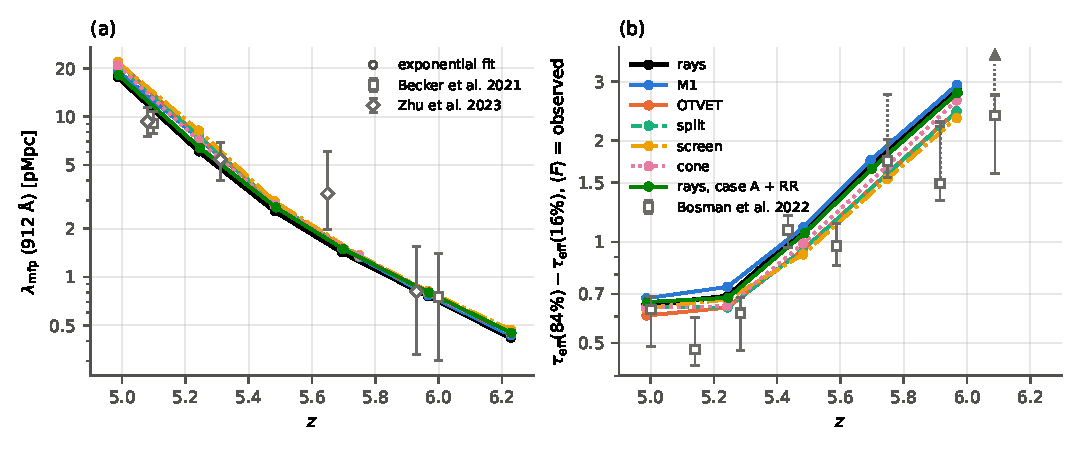
\includegraphics[width=\linewidth]{figures/fig_mfp_width.pdf}
\caption{The full-box snapshots of every run
(\texttt{scripts/fig\_mfp\_width.py}). (a) The 912\,\AA\ mean free path
from random starts (the distance where $\langle F\rangle=1/e$; open: the
exponential fit from ionised starts at $z\approx5$, where that distance
exceeds the sightlines), and the measurements of \citet{becker21} and
\citet{zhu23}. (b) The 84--16\% width of $\tau_{\rm eff}$ over $50\mpch$
segments ($3\times8192$ redshift-space skewers; a box-length skewer joined
to $10\mpch$ of another), with $\tau$ rescaled so that the mean flux
equals \citet{bosman22}'s.}
\label{fig:taueff}
\end{figure}



\appendix








%\begin{figure}[h]
%\centering
%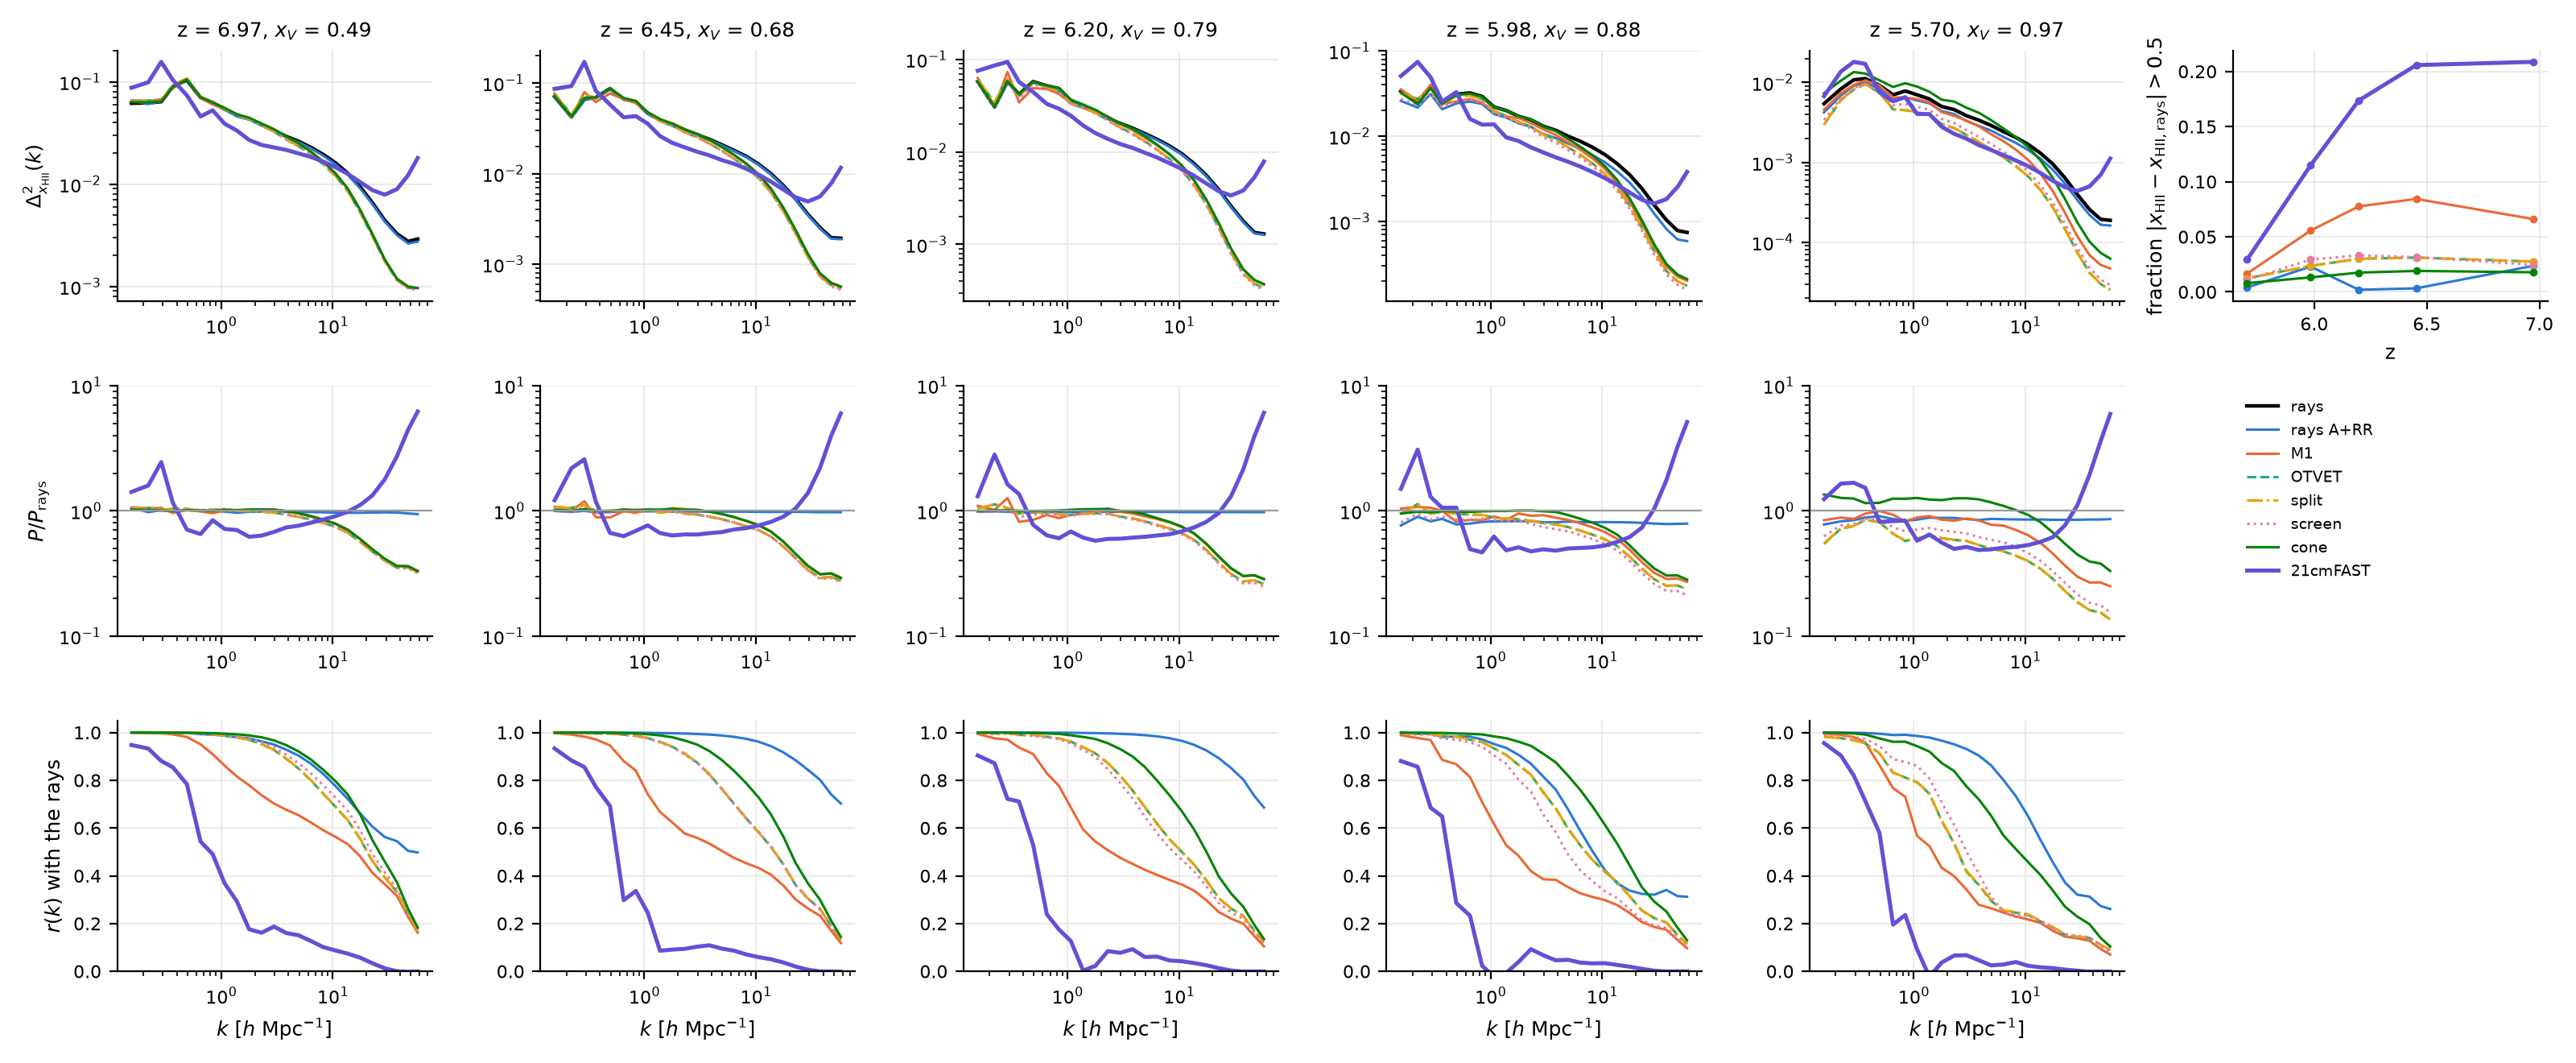
\includegraphics[width=\linewidth]{figures/fig8_21cmfast_pk_draft.png}
%\caption{21cmFAST (mass-dependent sources matched to the suite's,
%$R_{\rm max}=15$\,Mpc, on the suite's density; violet) against every RT
%method at the five snapshots during reionization: $\Delta^2$ of
%$x_{\rm HII}$, the ratio to the rays and $r(k)$ with them; top right, the
%fraction of cells whose $x_{\rm HII}$ differs from the rays' by more than
%0.5. \draft{NewRadHydroCode \texttt{taueff\_21cmfast\_fig8\_pk.png}
%(branch \texttt{21cmfast-mass-sources}, 61b8312); its colours differ from
%Figs.~\ref{fig:pkx}--\ref{fig:pkg} and are to be unified.}}
%\label{fig:21cmfast}
%\end{figure}

%======================================================================

\section{Cone parameters}
\begin{itemize}
\item nside 2$\to$4, receiver spacing 2$\to$4, $r_c$ 4$\to$8, the cutoff
  variants ($\lambda_x\in\{\infty,\lambda_{\rm eff},2\lambda_{\rm eff},$
  budget$\}$), blend $\sigma$: the \texttt{cmp\_*} tables of
  \texttt{docs/otvet\_closure.md} \S3.
\end{itemize}

\section{The minimum-image normalisation}\label{app:norm}
\begin{itemize}
\item $\int_{\rm cube}d^3r/(4\pi r^2)=0.610\,L$, so $L_O=4\pi\times0.610\,L=7.66\,L$
  in the notation of \citet{wu21}.
\item Box budget: $\sum N=q\sum L\,\lambda_{\rm eff}$,
  $\sum\Ndir=q\sum L\times0.61L$, so $\sum N/\sum\Ndir\approx\lambda_{\rm eff}/0.61L$.
\item Link to the $k$-independent amplitude ratio $4\pi\lambda/L_O$ of
  \citet{wu21}.
\end{itemize}






\bibliographystyle{plainnat}
\bibliography{refs}
\end{document}
